\documentclass{standalone}


\usepackage{tikz}
\usepackage{pgfplots}
\usetikzlibrary{calc}
\pgfplotsset{compat=1.15}

\begin{document}

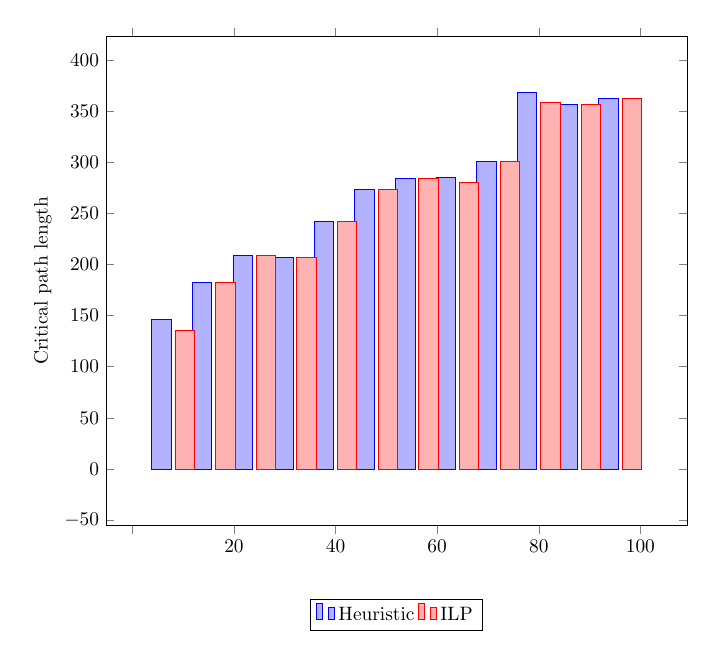
\begin{tikzpicture}[scale=0.7]
    \begin{axis}[
        width=\textwidth,
        ylabel=Critical path length,
				ymin=0,
				xticklabels={\null, \null,20, 40, 60, 80, 100, 120, 140, 160, 180, 200, 220, 240,\null},
        enlargelimits=0.15,
        legend style={at={(0.5,-0.15)},
        anchor=north,legend columns=-1},
        ybar,
        bar width=10pt,
        ]
        \addplot
        coordinates {
%(10 , 134)  
(20 , 146)  
%(30 , 163)  
(40 , 182) 
%(50 , 207) 
(60 , 209)  
%(70 , 206)  
(80 , 207)  
%(90 , 234)  
(100 , 242)  
%(110 , 249)  
(120 , 273)  
%(130 , 289)  
(140 , 284)  
%(150 , 268)  
(160 , 285)  
%(170 , 313)  
(180 , 301)  
%(190 , 333)  
(200 , 368)  
%(210 , 341)  
(220 , 356)  
%(230 , 337)  
(240 , 362)  
%(250 , 442) 
 
				};
        \addplot
        coordinates {
			%(10, 120)
(20, 135)
%(30, 163)
(40, 182)
%(50, 200)
(60, 209)
%(70, 205)
(80, 207)
%(90, 234)
(100, 242)
%(110, 247)
(120, 273)
%(130, 289)
(140, 284)
%(150, 268)
(160, 280)
%(170, 309)
(180, 301)
%(190, 333)
(200, 358)
%(210, 341)
(220, 356)
%(230, 336)
(240, 362)
%(250, 442)
				};
        
        \legend{Heuristic,ILP}
    \end{axis}
\end{tikzpicture}

\end{document}